\usetikzlibrary{calc,angles,quotes,arrows.meta,decorations.markings}



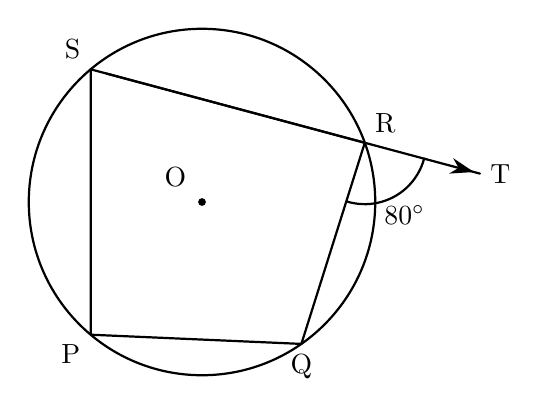
\begin{tikzpicture}[thick, line cap=round, line join=round, scale=1]

% ---------------------------
% Geometry setup (tuned to match the picture)
% ---------------------------
\coordinate (O) at (0,0);
\def\R{2.2}

% Points on the circle (chosen so PS is nearly vertical and PQ nearly horizontal)
\coordinate (S) at (130:\R);
\coordinate (P) at (230:\R);
\coordinate (Q) at (305:\R);
\coordinate (R) at (20:\R);

% T is on the extension of SR beyond R
\coordinate (T) at ($(S)!1.42!(R)$);

% ---------------------------
% Draw circle
% ---------------------------
\draw (O) circle (\R);

% Center dot and label
\fill (O) circle (1.4pt);
\node[above left=2pt] at (O) {O};

% ---------------------------
% Draw cyclic quadrilateral PQRS
% ---------------------------
\draw (P) -- (Q) -- (R) -- (S) -- cycle;

% ---------------------------
% Draw the extended chord SR to T
% Arrow placed near the tip (close to T), sitting on the line
% ---------------------------
\draw[
  shorten <=6pt, % keep arrow clear of the "T" label
  postaction={decorate},
  decoration={
    markings,
    mark=at position 0.985 with {\arrow{Stealth[length=3mm,width=2mm]}}
  }
] (S) -- (T);

% ---------------------------
% Angle arc at R between RQ and RT, labeled 80°
% ---------------------------
\pic[
  draw,
  angle radius=0.78cm,
  angle eccentricity=1.35,
  "$80^{\circ}$"
] {angle = Q--R--T};

% ---------------------------
% Labels positioned like the image
% ---------------------------
\node[above left]  at (S) {S};
\node[below left]  at (P) {P};
\node[below]       at (Q) {Q};
\node[above right] at (R) {R};
\node[right]       at (T) {T};

\end{tikzpicture}